\section{Design}

\begin{figure}[h]
\centering
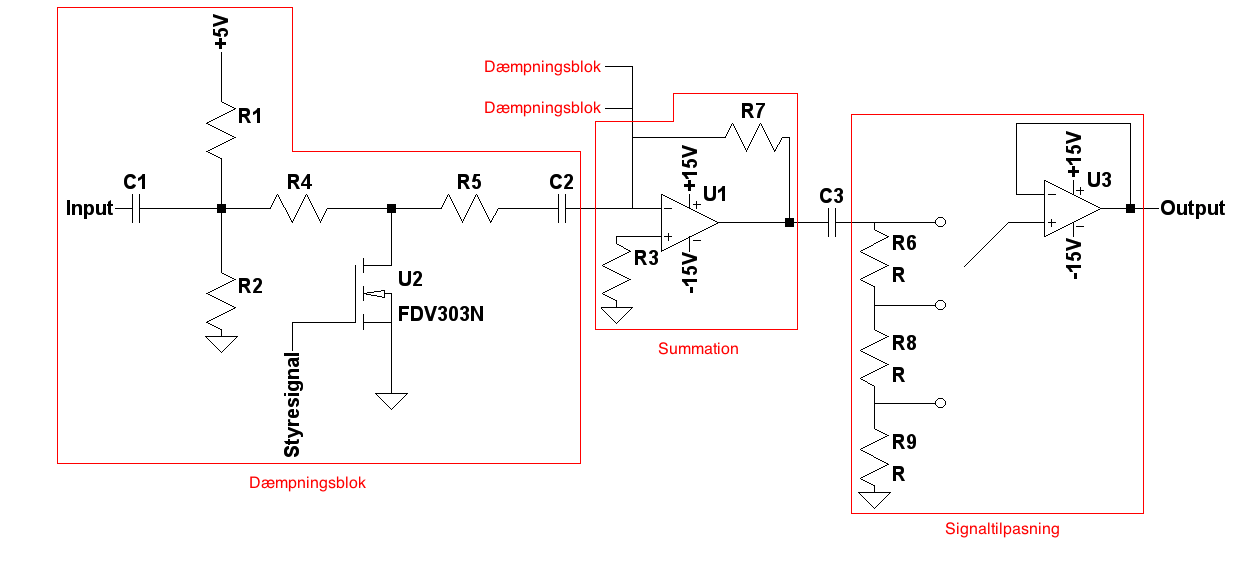
\includegraphics[width=\textwidth]{teknisk/indgangsvaelger/signal-taend-sluk.png}
\caption{Opbygning af indgangsvælgeren}
\label{fig:indgangsvaelger-overordnet}
\end{figure}

Indgangsvælgerkredsløbet kan opdeles i 3 sektioner: Dæmpningsblokke, summation og signaltilpasning. Diagrammet er vist på figur \ref{fig:indgangsvaelger-overordnet}. Dæmpningsblokkene sørger for at dæmpe signalet så meget som muligt, for at komme så tæt på en afkobling som muligt, når et signal skal slukkes. Summationssektionen lægger værdien af de foregående blokke sammen, mens signaltilpasningssektionen skifter mellem 3 forskellige niveauer, så det endelige output altid vil have et maksimalt peakniveau på 2 V.  

For at slukke signalet, er der valgt at benytte transistorer, til at trække signalerne til stel. Da spændingssvinget kan gå ned til 0,2 V, er der mulighed for at der vil løbe nogle små strømme i transistorerne. Derfor vælges en FET-transistor, da denne, modsat en BiPolær transistor, er linæer ved meget små collector-strømme\fixme{Hvor hen?}. For at aktivere transistoren, sættes spændingen på Gate-benet højt. Dette opnåes ved hjælp af et gatekredsløb. To D-flipflops opsættes til, ved hjælp af tryk på én enkelt knap, at skifte mellem fire forskellige binære tilstande. Opbygningen er vist på figur \ref{fig:indgangsvaelger-flipflop}. Disse fire tilstande repræsenterer de fire tilstande indgangsvælgeren kan være i: Begge tændt, begge slukket eller kun det ene signal tændt.

\begin{figure}[h]
\centering
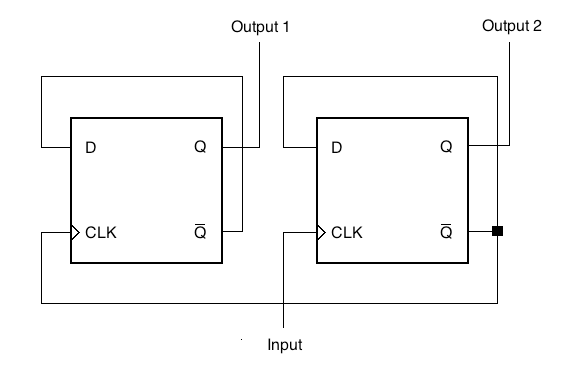
\includegraphics[scale=0.4]{teknisk/indgangsvaelger/flipflop.png}
\caption{Opbygning af indgangsvælgeren}
\label{fig:indgangsvaelger-flipflop}
\end{figure}

Optimalt ville en transistor uden reverse-diode være at foretrække, da dette vil tillade at source-spændingen er lavere end drainspændingen, som vil være tilfældet ved et AC-signal uden DC-offset. Da det ikke var muligt at fremskaffe en sådan, benyttes i stedet et DC-offset, til at sørge for at forskellen mellem DC-offsettet og AC-peakværdien er større end nul når transistoren er slukket, hvilket umuliggør at der kan løbe en reverse strøm i transistoren.

Modstandene $R_1$ og $R_2$ er begge valgt til 100~k\ohm, for at give et DC-offset på ca 2,5~V, halvdelen af 5~V, som vist på figur \ref{fig:indgangsvaelger-overordnet}. Dette gælder dog kun når transistoren er slukket. Idet transistoren tændes, sættes $R_2$ parallelt med $R_4$, hvilket trækker DC-offsettet længere ned.
%\begin{equation}
%5V\cdot \frac{\frac{1}{\frac{1}{R_2}+\frac{1}{R_3}}}{R_1+\frac{1}{\frac{1}{R_2}+\frac{1}{R_3}}}=1.11 V
%\end{equation}
I dette tilfælde, hvor transistoren skal trække signalet til stel, er DC-offsettet dog underordnet. 
Modstanden $R_3$ er valgt ud fra, at signalet skal se en indgangsimpedans på minimum 22 k\ohm. Når transistoren er tændt er indgangsimpedansen mindst. I denne situation sidder $R_1$, $R_2$ og $R_4$ parallelt, hvilket giver ligning (\ref{eq:indgangr4udregning}) og (\ref{eq:indgangr4}), forudsat at indgangsmodstanden er større end 22 k\ohm.

\begin{equation}
\label{eq:indgangr4udregning}
\frac{1}{\frac{1}{R_1}+\frac{1}{R_2}+\frac{1}{R_4}}=22~\mathrm{k}\ohm
\end{equation}

\begin{equation}
\label{eq:indgangr4}
R_4=39,29~\mathrm{k}\ohm
\end{equation}

For at kunne afbryde de enkelte signaler, kan transistoren $U_2$, på figur \ref{fig:indgangsvaelger-overordnet}, trække signalet til stel. Den fungerer i dette tilfælde som en switch, der skal tillade maksimal forbindelse mellem drain og source. For at tillade at hele signalet bliver trukket til stel, skal hele den strøm der løber igennem systemet føres ned igennem transistoren. På en MOSFET-transistor, som benyttes i dette kredsløb, løber der ingen strøm ind i gate, den er udelukkende afhængig af gate-source spændingen. Ved at påtrykke en spænding på 5 V, som er outputtet fra de gates der bruges, er det muligt at tillade signalet at løbe igennem transistoren.
Modstanden $R_5$ har ikke nogen indvirkning på indgangsimpedansen når transistoren er tændt og signalet derfor er slukket. Når signalet er tændt, sidder den i serie med $R_4$, hvilket giver en højere indgangsimpedans. For at summationsforstærkeren efter skal kunne fungere med en forstærkning på én, skal tilbagekoblingsmodstanden over transistoren være lig med den modstand signalet ser på vej til forstærkeren. Denne er afhængig af $R_4$ og $R_5$, som tilsammen skal give $R_7$. Med $R_7$ defineret til 80,4 k\ohm~sættes $R_5$ til 40,2 k\ohm. Indgangsimpedansen kan så udregnes, som i ligning (\ref{eq:indgangrindgang}).

%Den er valgt til 40.2 k\ohm, det samme som $R_3$, for at gøre produceringen enklere. Ved at bruge modstande med de samme værdier sænkes antallet af benyttede komponenter, hvilket letter indkøbs- samt produceringsomkostninger. Når signalet er tændt, sidder den i serie med $R_3$, hvilket giver en højere indgangsimpedans:

\begin{equation}
\label{eq:indgangrindgang}
R_{\mathrm{indgang}}=\frac{1}{\frac{1}{R_1}+\frac{1}{R_2}+\frac{1}{R_4 + R_5}}=30,8~\mathrm{k}\ohm
\end{equation}

Efter at have opstillet de forskellige modstandsværdier, er det muligt at udregne værdien af afkoblingskondensatorerne i kredsløbet. Disse kan udregnes som en spændingsdeling mellem en seriekoblet modstand og kondensator, seriekoblet med en modstand, som vist på figur \ref{crvd}.
\begin{figure}[h]
\centering
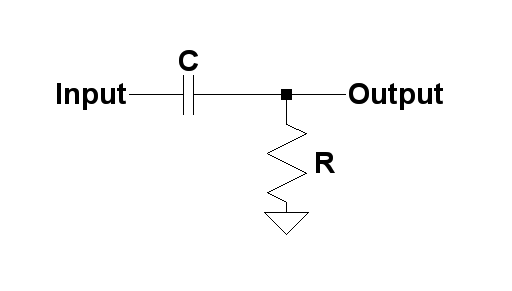
\includegraphics[scale=0.4]{teknisk/indgangsvaelger/hoejpasfilter.png}
\caption{Et standard CR højpasled}
\label{crvd}
\end{figure}
I dette tilfælde vil $R_U$ være udgangsimpedansen på det foregående led, og $R_I$ være indgangsimpedansen på det efterfølgende. Impedansen i en kondensator, i frekvensdomænet er $\frac{1}{s\cdot C}$. Dette kan opstilles ifølge spændingsdelingsformel som udtrykket i ligning (\ref{eq:indganghoejpas}).

\begin{equation}
\label{eq:indganghoejpas}
\frac{V_{\mathrm{out}}}{V_{\mathrm{in}}}=\frac{R_I}{R_I+\left(R_U+\frac{1}{s\cdot C}\right)}
\end{equation}

For at få en dæmpning på 3 dB, som er den ønskede dæmpning i knækfrekvensen, skal $\frac{V_{\mathrm{out}}}{V_{\mathrm{in}}}=10^{\frac{-3}{20}}\approx0,7$. 
Dette giver 2 ubekendte, $s$ og $C$. LaPlace variablen $s$ kan ses som $2\cdot \pi \cdot f$, hvor $f$ er den ønskede frekvens ved knækket, som vist i ligning (\ref{eq:indgang2pif}). Der opstilles et udtryk for $C$ i ligning (\ref{eq:indgangcudregning}).

\begin{equation}
\label{eq:indgang2pif}
10^{\frac{-3~\mathrm{dB}}{20}}=\frac{R_I}{R_I+\left(R_U+\frac{1}{2\cdot\pi\cdot 2~\mathrm{Hz}\cdot C}\right)}
\end{equation}

\begin{equation}
\label{eq:indgangcudregning}
C=\frac{-1}{2} \cdot 10^{\frac{-3~\mathrm{dB}}{20}} \pi \cdot f \cdot \left( 10^{\frac{-3~\mathrm{dB}}{20}} \cdot R_I + \frac{-3~\mathrm{dB}}{20} \cdot R_U - R_I \right)
\end{equation}

Frekvensen $f$ bestemmes til 2 Hz, én dekade før den ønskede, for at opnå en lav dæmpning ved de ønskede 20 Hz. Dæmpningen ved 20 Hz kan dermed udregnes. Formlen for et standard højpas-filter opstilles i formel (\ref{eq:indgangstandardhoejpas}). Denne omskrives så til $j\cdot\omega$-notation hvormed det ser ud som udtrykket i formel (\ref{eq:indgangjomega}).

\begin{equation}
\label{eq:indgangstandardhoejpas}
%\tau = R\cdot C
H(s)=\frac{s\cdot\tau}{1+s\cdot\tau}
\end{equation}

\begin{equation}
\label{eq:indgangjomega}
\left| H(j\omega) \right| = \frac{\omega\cdot\tau}{\sqrt{1+(\omega\cdot\tau)^2)}}=\frac{1}{\sqrt{\frac{1}{(\omega\cdot\tau)^2}+1}}
\end{equation}

Ifølge dekadereglen\fixme{måske en lille kilde ??}, sættes $\omega\cdot\tau = 10$, som i ligning (\ref{eq:indgangjomega10}).

\begin{equation}
\label{eq:indgangjomega10}
\frac{1}{\sqrt{\frac{1}{100}+1}}=\frac{1}{\sqrt{1,01}}\approx -0,043~\mathrm{dB}
\end{equation}

Ud fra dette kan de forskellige værdier for $C$ udregnes, afhængigt af de impedanser de ser ind i.
Impedansen, $C_1$ ser ind i, er fundet til 30,8 k\ohm . Indtastes dette i ovennævnte formel findes værdien for $C_1$ til mindst 8 µF. Alt under dette vil give en højere knækfrekvens, hvilket ikke er at ønske. Alt højere vil dog give en større indsvingningstid, hvilket, i forhold til en højere knækfrekvens, er at foretrække, dog heller ikke ønskeligt.
%$R_3$ skal være lig med den samlede impedans den minus porten på op-ampen kigger ind i. Denne udgøres af en parallel kobling af hver indgang og tilbagekoblingsmodstanden $R_7$, som vist i ligning \ref{eq:indgangr3}

%\begin{equation}
%\label{eq:indgangr3}
%R_3 = \frac{1}{\frac{1}{\frac{\frac{1}{\frac{1}{R_1}+\frac{1}{R_2}}+R_4+R_5}{3}}+\frac{1}{R_7}}
%\end{equation}

Efter summationsforstærkeren sidder signaltilpasningen. Denne benyttes til at sørge for at ligegyldigt hvor mange af indgangene der er tændt for, vil signalet altid have en peakspænding mellem 0,2 og 2 V. Da de niveauer der er mulige at få enten er 6, 4 eller 2 V, vil det for at give 2 V output, være nødvendigt med en dæmpning på hhv. $\frac{1}{3}$, $\frac{1}{2}$ og 1. Dette muliggøres ved hjælp af en spændingsdeler med 3 modstande, som vist under signaltilpasningsektionen af figur \ref{fig:indgangsvaelger-overordnet}. Værdierne af de forskellige modstande kan udregnes ud fra de givne modstandsforhold, som vist i ligning (\ref{eq:indgangsignal}). Modstande $R_9$ sættes til 10 k\ohm.
\begin{equation}
\label{eq:indgangsignal}
\frac{R_9}{R_6+R_8+R_9}=\frac{1}{2} \;\;\;\;\;\;\;\;\;\;\;\;~~~~~~~~~~~~~~~~
\frac{R_6+R_8}{R_6+R_8+R_9}=\frac{1}{3}
\end{equation}
Dette giver en $R_6$ på 15 k\ohm~og en $R_8$ på 5 k\ohm.
Vælgeren består af en multiplexer. Dette valg er taget på trods af valget om at designe primært med diskrete komponenter, da dette ville kunne gøres med stort set det samme kredsløb som indgangsvælgeren. \\Efter vælgeren sidder en buffer, for at impedansen der ses af afkoblingskondensatoren, som sidder mellem indgangsvælgeren og volumenkontrollen, vil være konstant.